% \documentclass[11pt]{article}

% % Change "review" to "final" to generate the final (sometimes called camera-ready) version.
% % Change to "preprint" to generate a non-anonymous version with page numbers.
% \usepackage[review]{acl}

% % Standard package includes
% \usepackage{times}
% \usepackage{latexsym}

% % For proper rendering and hyphenation of words containing Latin characters (including in bib files)
% \usepackage[T1]{fontenc}
% % For Vietnamese characters
% % \usepackage[T5]{fontenc}
% % See https://www.latex-project.org/help/documentation/encguide.pdf for other character sets

% % This assumes your files are encoded as UTF8
% \usepackage[utf8]{inputenc}

% % This is not strictly necessary, and may be commented out,
% % but it will improve the layout of the manuscript,
% % and will typically save some space.
% \usepackage{microtype}

% % This is also not strictly necessary, and may be commented out.
% % However, it will improve the aesthetics of text in
% % the typewriter font.
% \usepackage{inconsolata}

% %Including images in your LaTeX document requires adding
% %additional package(s)
% \usepackage{graphicx}

% % If the title and author information does not fit in the area allocated, uncomment the following
% %
% %\setlength\titlebox{<dim>}
% %
% % and set <dim> to something 5cm or larger.

% \title{Instructions for *ACL Proceedings}

% % Author information can be set in various styles:
% % For several authors from the same institution:
% % \author{Author 1 \and ... \and Author n \\
% %         Address line \\ ... \\ Address line}
% % if the names do not fit well on one line use
% %         Author 1 \\ {\bf Author 2} \\ ... \\ {\bf Author n} \\
% % For authors from different institutions:
% % \author{Author 1 \\ Address line \\  ... \\ Address line
% %         \And  ... \And
% %         Author n \\ Address line \\ ... \\ Address line}
% % To start a separate ``row'' of authors use \AND, as in
% % \author{Author 1 \\ Address line \\  ... \\ Address line
% %         \AND
% %         Author 2 \\ Address line \\ ... \\ Address line \And
% %         Author 3 \\ Address line \\ ... \\ Address line}

% \author{First Author \\
%   Affiliation / Address line 1 \\
%   Affiliation / Address line 2 \\
%   Affiliation / Address line 3 \\
%   \texttt{email@domain} \\\And
%   Second Author \\
%   Affiliation / Address line 1 \\
%   Affiliation / Address line 2 \\
%   Affiliation / Address line 3 \\
%   \texttt{email@domain} \\}

% %\author{
% %  \textbf{First Author\textsuperscript{1}},
% %  \textbf{Second Author\textsuperscript{1,2}},
% %  \textbf{Third T. Author\textsuperscript{1}},
% %  \textbf{Fourth Author\textsuperscript{1}},
% %\\
% %  \textbf{Fifth Author\textsuperscript{1,2}},
% %  \textbf{Sixth Author\textsuperscript{1}},
% %  \textbf{Seventh Author\textsuperscript{1}},
% %  \textbf{Eighth Author \textsuperscript{1,2,3,4}},
% %\\
% %  \textbf{Ninth Author\textsuperscript{1}},
% %  \textbf{Tenth Author\textsuperscript{1}},
% %  \textbf{Eleventh E. Author\textsuperscript{1,2,3,4,5}},
% %  \textbf{Twelfth Author\textsuperscript{1}},
% %\\
% %  \textbf{Thirteenth Author\textsuperscript{3}},
% %  \textbf{Fourteenth F. Author\textsuperscript{2,4}},
% %  \textbf{Fifteenth Author\textsuperscript{1}},
% %  \textbf{Sixteenth Author\textsuperscript{1}},
% %\\
% %  \textbf{Seventeenth S. Author\textsuperscript{4,5}},
% %  \textbf{Eighteenth Author\textsuperscript{3,4}},
% %  \textbf{Nineteenth N. Author\textsuperscript{2,5}},
% %  \textbf{Twentieth Author\textsuperscript{1}}
% %\\
% %\\
% %  \textsuperscript{1}Affiliation 1,
% %  \textsuperscript{2}Affiliation 2,
% %  \textsuperscript{3}Affiliation 3,
% %  \textsuperscript{4}Affiliation 4,
% %  \textsuperscript{5}Affiliation 5
% %\\
% %  \small{
% %    \textbf{Correspondence:} \href{mailto:email@domain}{email@domain}
% %  }
% %}

% \begin{document}
% \maketitle
% \begin{abstract}
% Please see the \LaTeX{} source of this document for comments on other packages that may be useful.


% \end{abstract}

% \section{Introduction}

% These instructions are for authors submitting papers to *ACL conferences using \LaTeX. They are not self-contained. All authors must follow the general instructions for *ACL proceedings,\footnote{\url{http://acl-org.github.io/ACLPUB/formatting.html}} and this document contains additional instructions for the \LaTeX{} style files.

% The templates include the \LaTeX{} source of this document (\texttt{acl\_latex.tex}),
% the \LaTeX{} style file used to format it (\texttt{acl.sty}),
% an ACL bibliography style (\texttt{acl\_natbib.bst}),
% an example bibliography (\texttt{custom.bib}),
% and the bibliography for the ACL Anthology (\texttt{anthology.bib}).

% \section{Engines}

% To produce a PDF file, pdf\LaTeX{} is strongly recommended (over original \LaTeX{} plus dvips+ps2pdf or dvipdf).
% The style file \texttt{acl.sty} can also be used with
% lua\LaTeX{} and
% Xe\LaTeX{}, which are especially suitable for text in non-Latin scripts.
% The file \texttt{acl\_lualatex.tex} in this repository provides
% an example of how to use \texttt{acl.sty} with either
% lua\LaTeX{} or
% Xe\LaTeX{}.

% \section{Preamble}

% The first line of the file must be
% \begin{quote}
% \begin{verbatim}
% \documentclass[11pt]{article}
% \end{verbatim}
% \end{quote}

% To load the style file in the review version:
% \begin{quote}
% \begin{verbatim}
% \usepackage[review]{acl}
% \end{verbatim}
% \end{quote}
% For the final version, omit the \verb|review| option:
% \begin{quote}
% \begin{verbatim}
% \usepackage{acl}
% \end{verbatim}
% \end{quote}

% To use Times Roman, put the following in the preamble:
% \begin{quote}
% \begin{verbatim}
% \usepackage{times}
% \end{verbatim}
% \end{quote}
% (Alternatives like txfonts or newtx are also acceptable.)

% Please see the \LaTeX{} source of this document for comments on other packages that may be useful.

% Set the title and author using \verb|\title| and \verb|\author|. Within the author list, format multiple authors using \verb|\and| and \verb|\And| and \verb|\AND|; please see the \LaTeX{} source for examples.

% By default, the box containing the title and author names is set to the minimum of 5 cm. If you need more space, include the following in the preamble:
% \begin{quote}
% \begin{verbatim}
% \setlength\titlebox{<dim>}
% \end{verbatim}
% \end{quote}
% where \verb|<dim>| is replaced with a length. Do not set this length smaller than 5 cm.

% \section{Document Body}

% \subsection{Footnotes}

% Footnotes are inserted with the \verb|\footnote| command.\footnote{This is a footnote.}

% \subsection{Tables and figures}

% See Table~\ref{tab:accents} for an example of a table and its caption.
% \textbf{Do not override the default caption sizes.}

% \begin{table}
%   \centering
%   \begin{tabular}{lc}
%     \hline
%     \textbf{Command} & \textbf{Output} \\
%     \hline
%     \verb|{\"a}|     & {\"a}           \\
%     \verb|{\^e}|     & {\^e}           \\
%     \verb|{\`i}|     & {\`i}           \\
%     \verb|{\.I}|     & {\.I}           \\
%     \verb|{\o}|      & {\o}            \\
%     \verb|{\'u}|     & {\'u}           \\
%     \verb|{\aa}|     & {\aa}           \\\hline
%   \end{tabular}
%   \begin{tabular}{lc}
%     \hline
%     \textbf{Command} & \textbf{Output} \\
%     \hline
%     \verb|{\c c}|    & {\c c}          \\
%     \verb|{\u g}|    & {\u g}          \\
%     \verb|{\l}|      & {\l}            \\
%     \verb|{\~n}|     & {\~n}           \\
%     \verb|{\H o}|    & {\H o}          \\
%     \verb|{\v r}|    & {\v r}          \\
%     \verb|{\ss}|     & {\ss}           \\
%     \hline
%   \end{tabular}
%   \caption{Example commands for accented characters, to be used in, \emph{e.g.}, Bib\TeX{} entries.}
%   \label{tab:accents}
% \end{table}

% As much as possible, fonts in figures should conform
% to the document fonts. See Figure~\ref{fig:experiments} for an example of a figure and its caption.

% Using the \verb|graphicx| package graphics files can be included within figure
% environment at an appropriate point within the text.
% The \verb|graphicx| package supports various optional arguments to control the
% appearance of the figure.
% You must include it explicitly in the \LaTeX{} preamble (after the
% \verb|\documentclass| declaration and before \verb|\begin{document}|) using
% \verb|\usepackage{graphicx}|.

% \begin{figure}[t]
%   \includegraphics[width=\columnwidth]{example-image-golden}
%   \caption{A figure with a caption that runs for more than one line.
%     Example image is usually available through the \texttt{mwe} package
%     without even mentioning it in the preamble.}
%   \label{fig:experiments}
% \end{figure}

% \begin{figure*}[t]
%   \includegraphics[width=0.48\linewidth]{example-image-a} \hfill
%   \includegraphics[width=0.48\linewidth]{example-image-b}
%   \caption {A minimal working example to demonstrate how to place
%     two images side-by-side.}
% \end{figure*}

% \subsection{Hyperlinks}

% Users of older versions of \LaTeX{} may encounter the following error during compilation:
% \begin{quote}
% \verb|\pdfendlink| ended up in different nesting level than \verb|\pdfstartlink|.
% \end{quote}
% This happens when pdf\LaTeX{} is used and a citation splits across a page boundary. The best way to fix this is to upgrade \LaTeX{} to 2018-12-01 or later.

% \subsection{Citations}

% \begin{table*}
%   \centering
%   \begin{tabular}{lll}
%     \hline
%     \textbf{Output}           & \textbf{natbib command} & \textbf{ACL only command} \\
%     \hline
%     \citep{Gusfield:97}       & \verb|\citep|           &                           \\
%     \citealp{Gusfield:97}     & \verb|\citealp|         &                           \\
%     \citet{Gusfield:97}       & \verb|\citet|           &                           \\
%     \citeyearpar{Gusfield:97} & \verb|\citeyearpar|     &                           \\
%     \citeposs{Gusfield:97}    &                         & \verb|\citeposs|          \\
%     \hline
%   \end{tabular}
%   \caption{\label{citation-guide}
%     Citation commands supported by the style file.
%     The style is based on the natbib package and supports all natbib citation commands.
%     It also supports commands defined in previous ACL style files for compatibility.
%   }
% \end{table*}

% Table~\ref{citation-guide} shows the syntax supported by the style files.
% We encourage you to use the natbib styles.
% You can use the command \verb|\citet| (cite in text) to get ``author (year)'' citations, like this citation to a paper by \citet{Gusfield:97}.
% You can use the command \verb|\citep| (cite in parentheses) to get ``(author, year)'' citations \citep{Gusfield:97}.
% You can use the command \verb|\citealp| (alternative cite without parentheses) to get ``author, year'' citations, which is useful for using citations within parentheses (e.g. \citealp{Gusfield:97}).

% A possessive citation can be made with the command \verb|\citeposs|.
% This is not a standard natbib command, so it is generally not compatible
% with other style files.

% \subsection{References}

% \nocite{Ando2005,andrew2007scalable,rasooli-tetrault-2015}

% The \LaTeX{} and Bib\TeX{} style files provided roughly follow the American Psychological Association format.
% If your own bib file is named \texttt{custom.bib}, then placing the following before any appendices in your \LaTeX{} file will generate the references section for you:
% \begin{quote}
% \begin{verbatim}
% \bibliography{custom}
% \end{verbatim}
% \end{quote}

% You can obtain the complete ACL Anthology as a Bib\TeX{} file from \url{https://aclweb.org/anthology/anthology.bib.gz}.
% To include both the Anthology and your own .bib file, use the following instead of the above.
% \begin{quote}
% \begin{verbatim}
% \bibliography{anthology,custom}
% \end{verbatim}
% \end{quote}

% Please see Section~\ref{sec:bibtex} for information on preparing Bib\TeX{} files.

% \subsection{Equations}

% An example equation is shown below:
% \begin{equation}
%   \label{eq:example}
%   A = \pi r^2
% \end{equation}

% Labels for equation numbers, sections, subsections, figures and tables
% are all defined with the \verb|\label{label}| command and cross references
% to them are made with the \verb|\ref{label}| command.

% This an example cross-reference to Equation~\ref{eq:example}.

% \subsection{Appendices}

% Use \verb|\appendix| before any appendix section to switch the section numbering over to letters. See Appendix~\ref{sec:appendix} for an example.

% \section{Bib\TeX{} Files}
% \label{sec:bibtex}

% Unicode cannot be used in Bib\TeX{} entries, and some ways of typing special characters can disrupt Bib\TeX's alphabetization. The recommended way of typing special characters is shown in Table~\ref{tab:accents}.

% Please ensure that Bib\TeX{} records contain DOIs or URLs when possible, and for all the ACL materials that you reference.
% Use the \verb|doi| field for DOIs and the \verb|url| field for URLs.
% If a Bib\TeX{} entry has a URL or DOI field, the paper title in the references section will appear as a hyperlink to the paper, using the hyperref \LaTeX{} package.

% \section*{Limitations}

% This document does not cover the content requirements for ACL or any
% other specific venue.  Check the author instructions for
% information on
% maximum page lengths, the required ``Limitations'' section,
% and so on.

% \section*{Acknowledgments}

% This document has been adapted
% by Steven Bethard, Ryan Cotterell and Rui Yan
% from the instructions for earlier ACL and NAACL proceedings, including those for
% ACL 2019 by Douwe Kiela and Ivan Vuli\'{c},
% NAACL 2019 by Stephanie Lukin and Alla Roskovskaya,
% ACL 2018 by Shay Cohen, Kevin Gimpel, and Wei Lu,
% NAACL 2018 by Margaret Mitchell and Stephanie Lukin,
% Bib\TeX{} suggestions for (NA)ACL 2017/2018 from Jason Eisner,
% ACL 2017 by Dan Gildea and Min-Yen Kan,
% NAACL 2017 by Margaret Mitchell,
% ACL 2012 by Maggie Li and Michael White,
% ACL 2010 by Jing-Shin Chang and Philipp Koehn,
% ACL 2008 by Johanna D. Moore, Simone Teufel, James Allan, and Sadaoki Furui,
% ACL 2005 by Hwee Tou Ng and Kemal Oflazer,
% ACL 2002 by Eugene Charniak and Dekang Lin,
% and earlier ACL and EACL formats written by several people, including
% John Chen, Henry S. Thompson and Donald Walker.
% Additional elements were taken from the formatting instructions of the \emph{International Joint Conference on Artificial Intelligence} and the \emph{Conference on Computer Vision and Pattern Recognition}.

% % Bibliography entries for the entire Anthology, followed by custom entries
% %\bibliography{anthology,custom}
% % Custom bibliography entries only
% \bibliography{custom}

% \appendix

% \section{Example Appendix}
% \label{sec:appendix}

% This is an appendix.

% \end{document}

% TEMPO-BIAS report — compiles with LuaLaTeX or XeLaTeX
\documentclass[11pt]{article}

\usepackage[review]{acl}
\usepackage{microtype}
\usepackage[english,bidi=default]{babel}
% Latin Modern Roman (bundled with TeX Live). For TeXGyre Termes X, use: \babelfont{rm}{TeXGyreTermesX}
\babelfont{rm}{Latin Modern Roman}

\usepackage{graphicx}
\usepackage{amsmath}
\usepackage{booktabs}

\title{Political Bias and Temporal Dynamics in Large Language Models}

\author{Ran Lu \\
  Université Paris-Saclay \\
  \texttt{ran.lu@universite-paris-saclay.fr} \\\And
  Hasti Hosseinpour \\
  Université Paris-Saclay \\
  \texttt{hasti.hosseinpour@universite-paris-saclay.fr} \\\And
  Abderrahmane Moujar \\
  Université Paris-Saclay \\
  \texttt{abderrahmane.moujar@universite-paris-saclay.fr} \\\And
  Oloruntobi Olutola \\
  Université Paris-Saclay \\
  \texttt{oloruntobi.olutola@universite-paris-saclay.fr}}

\begin{document}
\maketitle

\begin{abstract}
Large language models (LLMs) increasingly mediate how users access and interpret political information, yet most studies of political bias treat models as static. We study bias as a \emph{temporal} phenomenon using Prediction Inconsistency (IC) and sentiment label distributions on target-oriented classification. We evaluate two families---OpenAI ChatGPT (gpt-3.5-turbo through gpt-4o) and Meta Llama~3.2 (Base and Instruct, 1B--11B)---on fixed entities and templates. For ChatGPT, IC rises from near zero (gpt-3.5-turbo) to $\approx$0.67 (gpt-4) and plateaus at $\approx$0.61 for later variants; labels shift from 100\% positive to a mix of positive and UNKNOWN. For Llama, IC is lower (0.005--0.178); instruction tuning sharply reduces IC for 1B and yields minimal inconsistency for the 11B vision model. We show that political bias, as captured by IC and label distribution, evolves with model family, version, and alignment, and argue for longitudinal evaluation in bias research.
\end{abstract}

\section{Introduction}

Large language models have become central intermediaries in how people access, interpret, and evaluate political information. Their use in summarization, question answering, and sentiment analysis gives them substantial influence over public discourse. A growing body of work demonstrates that LLMs are not ideologically neutral: political tendencies emerge from training data, architecture, and alignment \citep{santurkar2023,buyl2026,hartmann2023,bang2024}. When models systematically favor or disfavor certain actors or viewpoints, they can function as implicit instruments of political influence.

Most prior work evaluates political bias at a single point in time. This static view is increasingly inadequate. Model families such as LLaMA and GPT evolve rapidly; training corpora, safety data, and alignment procedures change across generations \citep{touvron2023,dubey2024}. Such interventions may affect not only safety and factuality but also political framing and sentiment. We therefore study political bias through a \emph{temporal} lens: how does it change across model generations and alignment stages?

We adopt the framework of \citet{elbouanani2025}, who quantify bias via Prediction Inconsistency (IC)---the instability of sentiment predictions when the target political entity is swapped in a sentence. We extend this to a longitudinal setting and evaluate two families: OpenAI ChatGPT (five versions from gpt-3.5-turbo to gpt-4o) and Meta Llama~3.2 (Base and Instruct, including 1B, 3B, and 11B vision). Our research questions are: (1) How does IC evolve across model versions? (2) How does alignment (Base vs.\ Instruct) affect IC and sentiment label distribution? (3) How do these patterns differ across families?

Our contributions are: (i) a temporal view of political bias in LLMs; (ii) longitudinal IC and label-distribution results for ChatGPT and Llama on the same task; and (iii) evidence that the effect of alignment on bias is size- and family-dependent.

\section{Related Work}

Political bias in LLMs has been studied along several axes. Early work mapped model outputs onto ideological frameworks \citep{santurkar2023,hartmann2023}. Later studies distinguished explicit stance from framing and lexical polarity \citep{bang2024} and operationalized bias via target-oriented sentiment classification \citep{wang2025,chen2024}. \citet{elbouanani2025} introduce Prediction Inconsistency (IC) as the entropy of predicted labels across entity substitutions; we adopt this metric and extend it to a temporal setting.

Temporal drift in LLM behavior and bias is well documented \citep{zhu2024,buyl2026}. Technical reports on LLaMA describe substantial changes in safety data and alignment across generations \citep{touvron2023,dubey2024}; comparative evaluations show that newer models handle politically nuanced content differently \citep{crum2024}. Mitigation and alignment can alter political nuance \citep{banko2025,bonaldi2024}. We contribute a direct, longitudinal comparison of IC and label distributions across ChatGPT and Llama under controlled prompts and entities.

\section{Methodology}

We follow \citet{elbouanani2025}. \textbf{Data.} We use 250 political entities from major regions and 60 sentence templates (positive, neutral, negative). Entity names are substituted into templates; the only varying factor per prompt is the entity. \textbf{Task.} Target-oriented sentiment classification (TSC): models predict one of \{\text{positive}, \text{neutral}, \text{negative}\}. \textbf{Metric.} Prediction Inconsistency (IC). For each template $s$, we obtain a distribution over labels across entities:
$P(l|s) = |\{e \in E : \text{pred}(s,e)=l\}|/|E|$. The entropy $H(s) = -\sum_l P(l|s)\log P(l|s)$ measures inconsistency for that template; we report the average over templates: $\text{IC} = \frac{1}{m}\sum_i H(s_i)$. IC = 0 corresponds to perfectly consistent (unbiased) predictions.

\textbf{Setup.} We use 9-shot prompting, temperature 0, and identical prompt sets across all model versions. \textbf{Models.} ChatGPT: gpt-3.5-turbo, gpt-4, gpt-4-turbo, gpt-4o-mini, gpt-4o. Llama~3.2: Base (1B, 3B text-q8\_0); Instruct (1B, 3B, vision 11B).

\section{Results}

Figure~\ref{fig:results} summarizes IC across versions. We report IC and label distributions below.

\subsection{ChatGPT}

IC is near zero for \textbf{gpt-3.5-turbo}. It jumps to $\approx$0.67 for \textbf{gpt-4} (the highest among all versions) and then plateaus at $\approx$0.61 for \textbf{gpt-4-turbo}, \textbf{gpt-4o-mini}, and \textbf{gpt-4o} (overall mean 0.501). Thus the main increase in political bias, as measured by IC, occurs at the transition from gpt-3.5-turbo to gpt-4; later gpt-4-family models maintain high but slightly lower inconsistency.

Label distributions shift sharply. Gpt-3.5-turbo assigns \textbf{100\% positive}; no neutral, negative, or UNKNOWN. Gpt-4 gives $\approx$60\% positive and $\approx$40\% UNKNOWN. Gpt-4-turbo, gpt-4o-mini, and gpt-4o each give $\approx$30\% positive and $\approx$70\% UNKNOWN. None of the models output neutral or negative in this evaluation. The rise in UNKNOWN in the gpt-4 family may reflect greater refusal or hedging, while still producing high inconsistency when the entity is varied.

\subsection{Llama}

\textbf{Pre-trained (Base).} IC decreases with size: 1B $\approx$0.178, 3B $\approx$0.118. \textbf{Post-trained (Instruct).} 1B has IC $\approx$0.028 (much lower than Base); 3B remains $\approx$0.120 (similar to Base); vision 11B has the lowest IC ($\approx$0.005). Instruction tuning therefore strongly reduces IC for the 1B model and yields minimal inconsistency for the 11B vision model; the 3B model is largely unchanged by alignment.

Label distributions differ by size and stage. Base 1B/3B skew negative; Instruct 1B becomes $\approx$97--98\% negative. Instruct 3B shows more positive and neutral (e.g., $\approx$52\% positive, 10\% neutral, 36\% negative); Instruct vision 11B is more balanced ($\approx$32\% positive, 30\% neutral, 34\% negative). Alignment thus shifts sentiment distributions in a size-dependent way.

\subsection{Cross-family comparison}

ChatGPT exhibits higher IC (0.61--0.67) than the Llama models we evaluated (0.005--0.178). ChatGPT outputs are dominated by positive and UNKNOWN; Llama models produce substantial negative and neutral shares. Political bias, as captured by IC and label distribution, therefore varies by family, version, and alignment.

\begin{figure*}[t]
  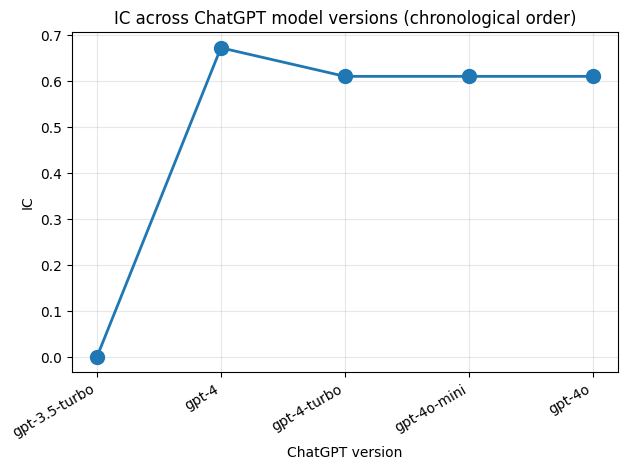
\includegraphics[width=0.48\textwidth]{../figures/chatgpt_ic_chronological.png}
  \hfill
  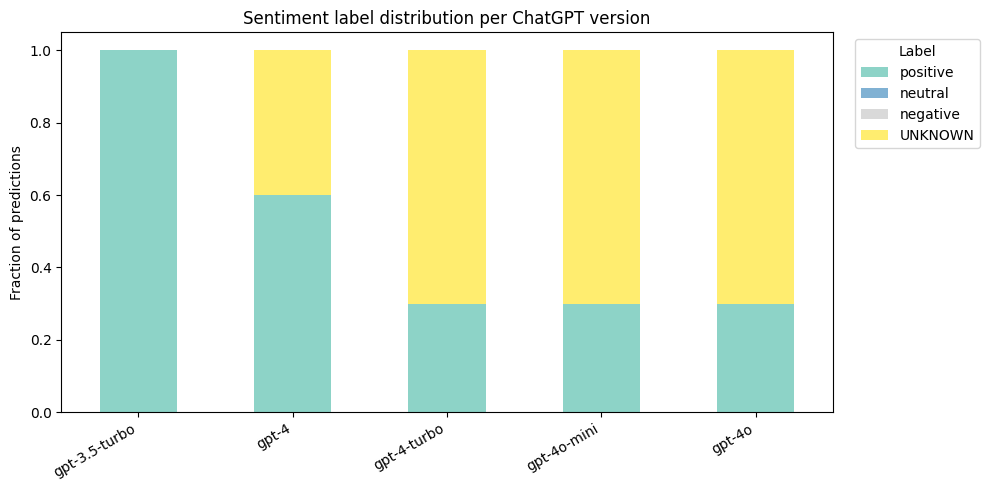
\includegraphics[width=0.48\textwidth]{../figures/llama_ic_base_instruct.png}
  \caption{Left: IC across ChatGPT versions (chronological). Right: IC for Llama~3.2 Base vs.\ Instruct.}
  \label{fig:results}
\end{figure*}

\section{Discussion and Conclusion}

Our results show that political bias in LLMs is not static. For ChatGPT, IC rises sharply with gpt-4 and then plateaus; the shift from all-positive to large UNKNOWN shares may reflect different refusal or classification behavior while still yielding high inconsistency. For Llama, instruction tuning reduces IC for the 1B and 11B vision models but not for 3B; sentiment distributions change markedly with alignment and size. Cross-family, ChatGPT has higher IC and different label patterns than Llama, underscoring that bias is family- and alignment-dependent.

\textbf{Limitations.} We evaluate two families and a fixed set of versions; results may not generalize. IC captures prediction inconsistency under entity substitution but not other dimensions of bias (e.g., framing or ideological stance). The high share of UNKNOWN for some ChatGPT versions complicates interpretation. Differences in API behavior and model access may confound cross-model comparison.

\textbf{Future work.} Extend to more families, longer time horizons, and other bias metrics; relate IC to fairness and stance measures.

\section*{Acknowledgments}
We thank Prof. Adrian Popescu (Fairness in AI, Université Paris-Saclay) and the TEMPO-BIAS project.

\bibliography{custom}

\end{document}

